%-------------------------------%
% Template modify from Alexander Soen's Student Assignment Template
%https://www.overleaf.com/latex/templates/student-assignment-template/sjkprrdkmphg
%-------------------------------%

\documentclass[a4paper]{article}
\usepackage{student}
\usepackage{float}

% Metadata
\date{\today}
\setmodule{Assignment 3 Report}
\setterm{114-1 (Fall 2025)}

%-------------------------------%
% Other details
% TODO: Fill the information
%-------------------------------%
\title{Reinforcement Learning}
\setmembername{Ivan Chang} % In English
\setmemberuid{B13901165}
%-------------------------------%
% Add / Delete commands and packages
% TODO: Add / Delete here as you need
%-------------------------------%
\usepackage{amsmath,amssymb,bm}
\usepackage{graphicx}
\usepackage{caption}
\usepackage{subcaption}
\usepackage{float}

\newcommand{\KL}{\mathrm{KL}}
\newcommand{\R}{\mathbb{R}}
\newcommand{\E}{\mathbb{E}}
\newcommand{\T}{\top}

\newcommand{\expdist}[2]{%
        \normalfont{\textsc{Exp}}(#1, #2)%
    }
\newcommand{\expparam}{\bm \lambda}
\newcommand{\Expparam}{\bm \Lambda}
\newcommand{\natparam}{\bm \eta}
\newcommand{\Natparam}{\bm H}
\newcommand{\sufstat}{\bm u}

% Main document
\begin{document}
    % Add header
    \header{}

    % Use `answer` environment to add solutions
    % \begin{answer}[Question 1.1] for example starts an environment formatted
    % for Question 1.1
    \begin{answer}[Q1. Try using at least two different algorithms to train your 2048 model. Present your results and discuss possible reasons why some algorithms perform better than others in this task. (12 pts.) ]
        In my experiments, I have tried DQN and PPO to train the 2048 model.
    \subsection{Hyperparameters}
        \begin{itemize}
            \item policy\_network: CnnPolicy
            \item num\_train\_envs: 6
            \item epoch\_num: 1000
            \item timesteps\_per\_epoch: 2048*6*2
            \item eval\_episode\_num: 10
            \item ent\_coef: 0.025
        \end{itemize}
    \subsection{Training Results}
    \begin{figure}[H]
        \centering
        \includegraphics[width=0.6\textwidth]{avg\_highest.png}
        \caption{avg\_highest\_tile vs number of epochs}
    \end{figure}
    \begin{figure}[H]
        \centering
        \includegraphics[width=0.6\textwidth]{avg\_score.png}
        \caption{avg\_score vs number of epochs}
    \end{figure}
    \subsection{Discussion}
    As you can see from the training results, DQN outperforms PPO significantly in both average highest tile and average score. PPO can barely be trained.
    First, we have to think about the characteristiccs of 2048 game. 
    \begin{itemize}
        \item Both the state space and the action space are discrete. 
        \item The state space is huge while the action space is small (4 actions).
        \item The environment is stochastic since the new tiles are randomly generated.
    \end{itemize}
    During my experiments, I find out that DQN performs much better than PPO in this task.
    I assume that the possible reasons are as follows:
    \begin{itemize}
        \item DQN is designed for discrete action space, while PPO is more general and can handle both discrete and continuous action spaces. But the continuous action is meaningless in 2048.
        so the policy output from PPO may not be very useful.
        \item The merge reward is exponentially increasing, which leads to high variance in PPO's policy gradient estimates. 
        DQN, on the other hand, uses Q-learning and square loss, which can be more stable in such scenarios.
        \item DQN uses experience replay, which can reuse past data and improve sample efficiency. PPO, which is an on-policy method, cannot benefit from this.
    \end{itemize}
    \end{answer}

    \begin{answer}[Q2. Show your best tile distribution in 2048 (8 pts.)]
        My model can reach 2048 tile with the probability of approximately 6\% to 7\% after training. 
        The distribution of the highest tiles achieved over 100 evaluation episodes is shown in the following figure.
        \begin{figure}[H]
            \centering
            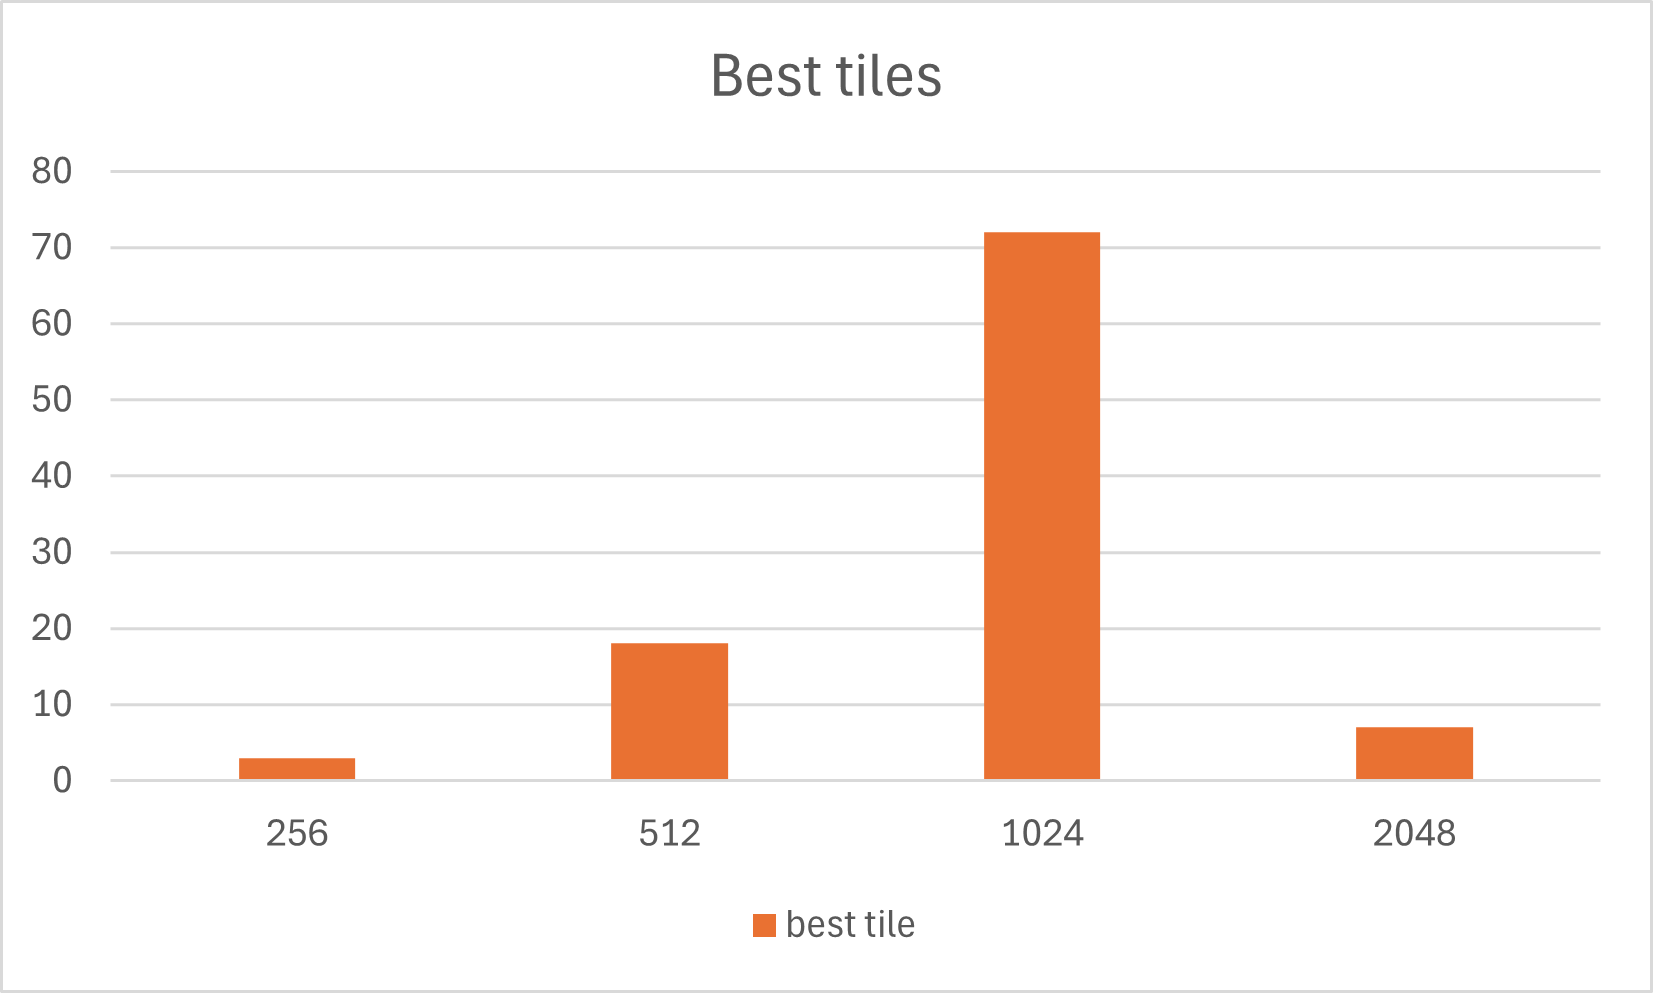
\includegraphics[width=0.6\textwidth]{best_tile.png}
            \caption{Distribution of highest tiles over 100 evaluation episodes}
        \end{figure}
        \begin{figure}[H]
            \centering
            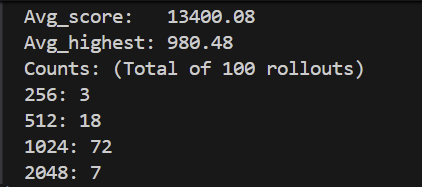
\includegraphics[width=0.6\textwidth]{best_tile_original_data.png}
            \caption{Original output}
        \end{figure}
    \end{answer}
    \begin{answer}[Q3. Describe what you have done to train your best model (10 pts.)]
        I will discuss this part into two sections: algorithm and reward shaping.
        \subsection{Algorithm}
        I refer to the neural network structure proposed in the paper "Developing Value Networks for Game 2048
with Reinforcement Learning" which uses convolutional layers and fully connected layers to capture the spatial features of the board.:
        \begin{table}[H]
            \centering
            \caption{Architecture of CNN22 Network}
            \begin{tabular}{clcc}
                \hline
                Layer & Type & Filters / Neurons & Activation \\ \hline
                1 & Convolution (2$\times$2) & 256 & ReLU \\
                2 & Convolution (2$\times$2) & 512 & ReLU \\
                3 & Fully Connected & 1024 & ReLU \\
                4 & Fully Connected & 256 & ReLU \\
                5 & Fully Connected (Output Value) & 1 & None \\ \hline
            \end{tabular}
        \end{table}
        Since we have to capture the spatial feature of the board, convolution layers are more suitable than fully connected layers.
        Also, 2x2 filters are used to capture the local patterns of tile merging.
        \subsection{Reward Shaping}
        As for the reward shaping, I have adjust a few parts:
        \begin{itemize}
            \item Instead of directly finalizing the game when model performs an illegal move, I give 
            them five chances to make illegal moves before ending the game(with huge penalty). This allows the model to explore more states.
            \item I notice that experts usually put the highest tile in the corner. Therefore, I give extra rewards if the highest tile is in the corner.
            \item During the game, we should maintain the monotonicity of the tiles. I focus on the last row and give extra rewards for monotonicity
            \item if the last row is full, the largest tile would not be moved with the left action. Therefore, I give extra rewards if the last row is full.
        \end{itemize}

    \end{answer}
    \begin{answer}[Q4. Choose an environment from the Gymnasium library (cannot be 2048) and train an agent. Show your results and write down anything you find interesting or difficult using pen and paper, and include a photo or a scan of it. (10 pts.)]
        \subsection{Discussion}
        I have chosen the \textbf{frozen lake} environment from the Gymnasium library. which requires the agent to cross a frozen lake without
        falling into the holes. Due to the discrete and small state space, I simply use traditional tabular RL with Q-learning algorithm to train the agent.
        the parameters are shown as follows:
        \begin{itemize}
            \item learning rate: 0.1
            \item discount factor: 0.99
            \item exploration rate: starting from 1.0 and decay to 0.1
        \end{itemize}

        After training for 15000 episodes, the agent can reach the end point with a success rate of 100\% which indicates that the agent has learned the optimal policy.
        \begin{figure}[H]
            \centering
            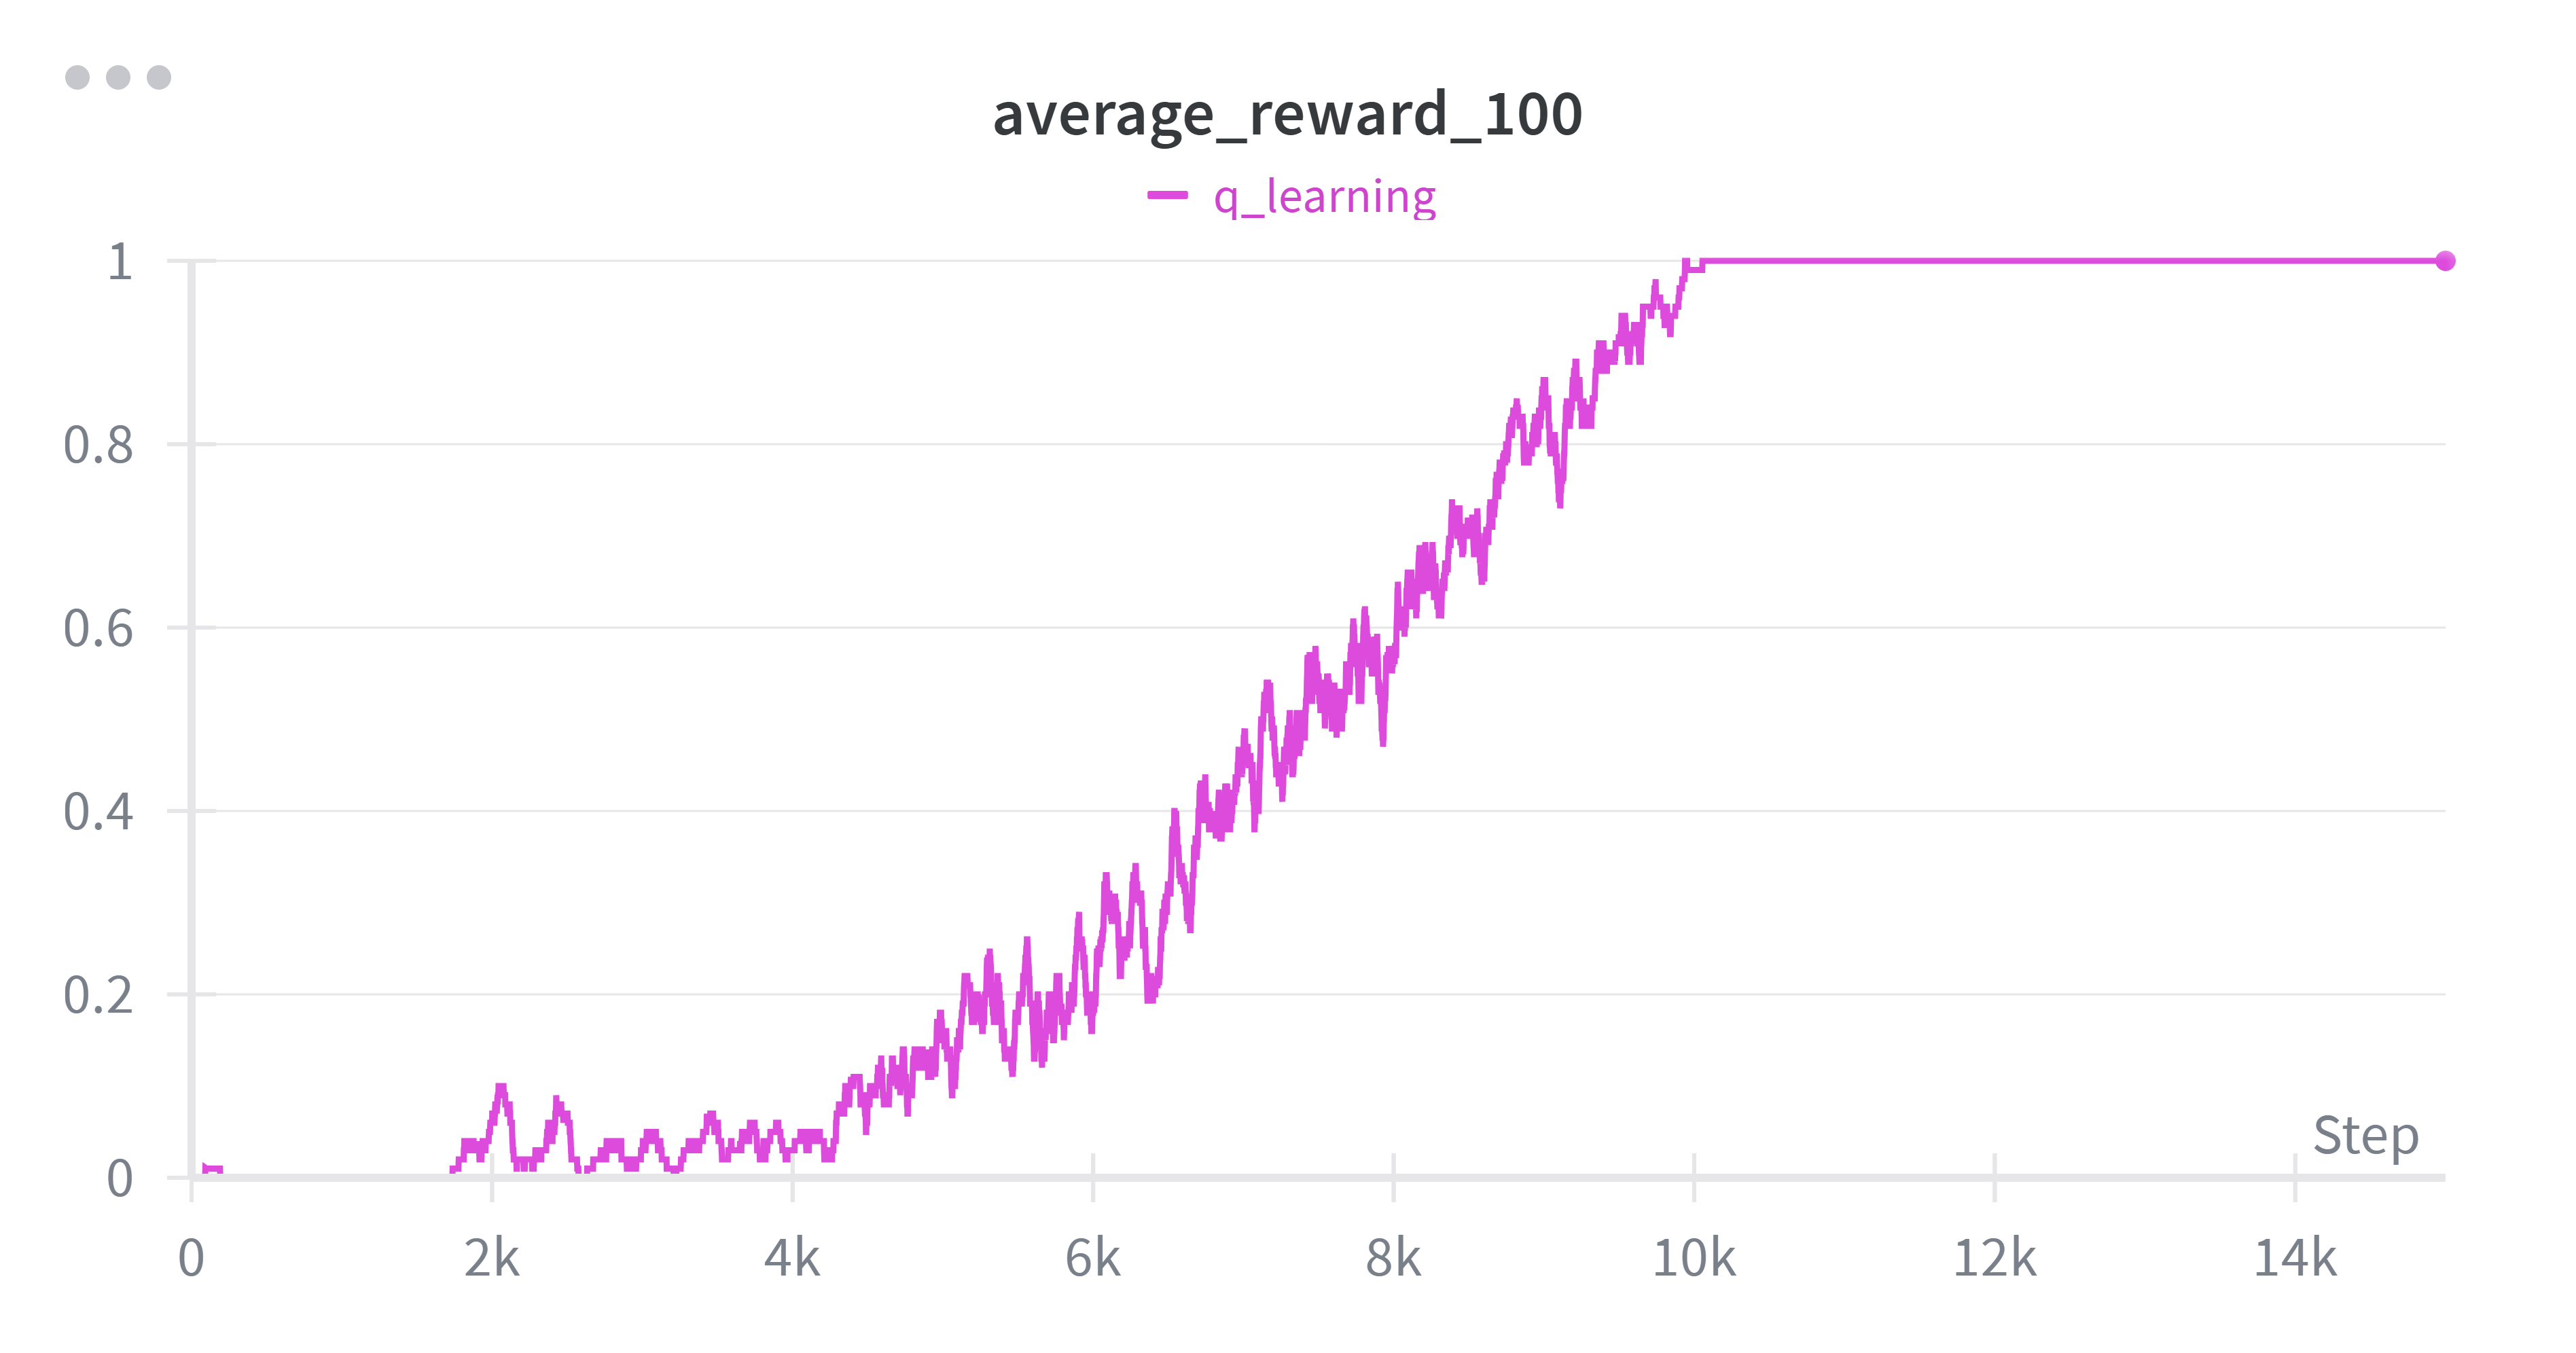
\includegraphics[width=0.6\textwidth]{frozen_lake.png}
            \caption{success rate over the last 100 episodes during training vs number of episodes}
        \end{figure}
        \subsection{Reflection}
        \begin{figure}[H]
            \centering
            \includegraphics[angle=180, width=0.6\textwidth]{hand_written.jpg}
            \caption{My pen-and-paper notes on the Frozen Lake environment}
        \end{figure}
    \end{answer}
\end{document}
